
% This LaTeX was auto-generated from MATLAB code.
% To make changes, update the MATLAB code and republish this document.

\documentclass{article}
\usepackage{graphicx}
\usepackage{color}

\sloppy
\definecolor{lightgray}{gray}{0.5}
\setlength{\parindent}{0pt}

\begin{document}

    
    
\section*{Aproximare MCMMP}


\subsection*{Contents}

\begin{itemize}
\setlength{\itemsep}{-1ex}
   \item Recens\u{a}m\^{a}ntul SUA
   \item Fitting direct
   \item Fitting cu date normalizate
\end{itemize}


\subsection*{Recens\u{a}m\^{a}ntul SUA}

\begin{par}
Datele de mai jos au fost \^{\i}nregistrate de US Census \^{\i}ntre 1900 \c{s}i 2010
\end{par} \vspace{1em}
\begin{verbatim}
%CENSUS - example with census data
%          polynomial fit

%population
y = [ 75.995  91.972 105.711 123.203 131.669 150.697 ...
    179.323 203.212 226.505 249.633 281.422 308.786]';

t = (1900:10:2010)';   % census years
\end{verbatim}
\begin{par}
Dorim sa model\u{a}m datele \c{s}i s\u{a} facem predic\c{t}ii pentru anii 1975 \c{s}i 2015
\end{par} \vspace{1em}
\begin{verbatim}
x = (1890:1:2019)';    % evaluation years
w = [1975,2015];       % prediction years
\end{verbatim}
\begin{par}
Vom modela datele printr-un polinom de gradul 3
\end{par} \vspace{1em}
\begin{par}
$$y=c_{1}t^3+c_{2}t^2+c_{3} t+c_{4}$$
\end{par} \vspace{1em}


\subsection*{Fitting direct}

\begin{verbatim}
c=polyfit(t,y,3)
\end{verbatim}

        \color{lightgray} \begin{verbatim}Warning: Polynomial is badly conditioned. Add points with distinct X values,
reduce the degree of the polynomial, or try centering and scaling as described
in HELP POLYFIT. 

c =

  -6.5861e-06     0.047733         -109        80029

\end{verbatim} \color{black}
    \begin{par}
Rezultatele sunt inacceptabile din punct de vedere numeric.
\end{par} \vspace{1em}
\begin{par}
Vom normaliza datele cu
\end{par} \vspace{1em}
\begin{par}
$$s=\frac{t-\bar{t}}{\sigma(t)}$$
\end{par} \vspace{1em}
\begin{verbatim}
mt=mean(t); st=std(t);

s=(t-mt)/st;
xs=(x-mt)/st;
\end{verbatim}


\subsection*{Fitting cu date normalizate}

\begin{par}
coeficien\c{t}ii
\end{par} \vspace{1em}
\begin{verbatim}
cs=polyfit(s,y,3)
\end{verbatim}

        \color{lightgray} \begin{verbatim}
cs =

     -0.30871       11.837       76.561       166.49

\end{verbatim} \color{black}
    \begin{par}
predic\c{t}iile
\end{par} \vspace{1em}
\begin{verbatim}
zs=polyval(cs,xs);
est=polyval(cs,(w-mt)/st);
\end{verbatim}
\begin{par}
reprezentare grafic\u{a}
\end{par} \vspace{1em}
\begin{verbatim}
plot(t,y,'o',x,zs,'-',w,est,'*')
for i=1:length(w)
    text(w(i),est(i)-20,num2str(est(i)))
end
title('U.S. Population', 'FontSize', 14)
xlabel('year', 'FontSize', 12)
ylabel('Millions', 'FontSize', 12)
\end{verbatim}

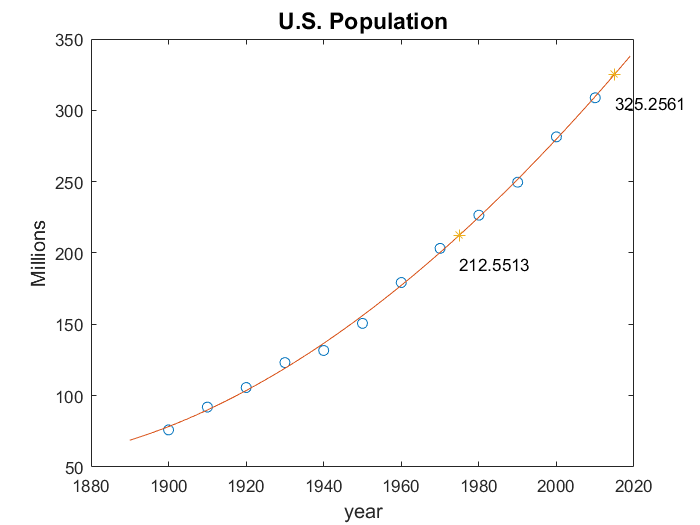
\includegraphics [width=4in]{census2b_01.png}



\end{document}
    
